\documentclass[border=2pt]{standalone}
\usepackage[dvipsnames,svgnames,x11names]{xcolor}
\usepackage{tikz}
\usetikzlibrary{arrows.meta,backgrounds,fit}
\begin{document}
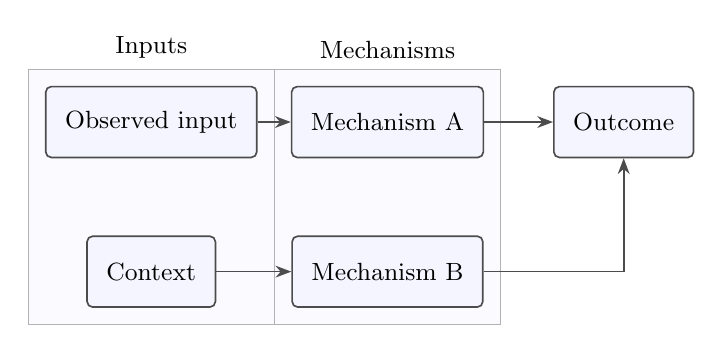
\begin{tikzpicture}[font=\small,>=Stealth,x=30mm,y=19mm]
\node[rectangle,rounded corners=2pt,fill=blue!4,draw=black!70,text=black,line width=0.6pt,minimum height=9mm,inner xsep=7pt,inner ysep=4.5pt,align=center] (x1) at (0,0) {Observed input};
\node[rectangle,rounded corners=2pt,fill=blue!4,draw=black!70,text=black,line width=0.6pt,minimum height=9mm,inner xsep=7pt,inner ysep=4.5pt,align=center] (x2) at (0,-1) {Context};
\node[rectangle,rounded corners=2pt,fill=blue!4,draw=black!70,text=black,line width=0.6pt,minimum height=9mm,inner xsep=7pt,inner ysep=4.5pt,align=center] (m1) at (1,0) {Mechanism A};
\node[rectangle,rounded corners=2pt,fill=blue!4,draw=black!70,text=black,line width=0.6pt,minimum height=9mm,inner xsep=7pt,inner ysep=4.5pt,align=center] (m2) at (1,-1) {Mechanism B};
\node[rectangle,rounded corners=2pt,fill=blue!4,draw=black!70,text=black,line width=0.6pt,minimum height=9mm,inner xsep=7pt,inner ysep=4.5pt,align=center] (y) at (2,0) {Outcome};
\begin{scope}[on background layer]
\node[fit=(x1)(x2),inner sep=6pt,fill=blue!2,draw=black!30,line width=0.45pt,label={[font=\small]above:{Inputs}}] (inputs) {};
\node[fit=(m1)(m2),inner sep=6pt,fill=blue!2,draw=black!30,line width=0.45pt,label={[font=\small]above:{Mechanisms}}] (mechanisms) {};
\end{scope}
\draw[->,draw=black!70,line width=0.6pt] (x1) -- (m1);
\draw[->,draw=black!70,line width=0.6pt] (x2) -- (m2);
\draw[->,draw=black!70,line width=0.6pt] (m1) -- (y);
\draw[->,draw=black!70,line width=0.6pt] (m2) -| (y);
\end{tikzpicture}
\end{document}
